\documentclass{report}

\usepackage[utf8]{inputenc}
\usepackage[document]{ragged2e}
\usepackage{Sweave}
\begin{document}
\Sconcordance{concordance:rapport_latex.tex:rapport_latex.Rnw:%
1 4 1 1 0 25 1 1 9 19 1 1 4 3 1 1 4 4 1 1 4 111 0 1 2 15 1 1 4 18 0 1 2 %
13 1 1 5 10 1 1 4 25 0 1 3 1 0 1 2 1 7 1 2 10 1 1 29 1 2 5 1 1 5 1 2 8 %
1}


\begin{titlepage}
    \begin{center}
        \vspace*{1cm}
 
        \Huge
        \textbf{Machine learning - DTU}
 
        \vspace{0.5cm}
        \LARGE
        Rapport 
 
        \vspace{1.5cm}
 
        \textbf{Anna Louise Hansen}
        \vfill
 
        Fra Udviklings- og Forenklingsstyrrelsen
 
        \vspace{0.8cm}
 
    \end{center}
\end{titlepage}



\chapter{Part I}

\section{Beskrivelse af data}
Alle boligejere i Danmark betaler en skat, ejendomsværdiskat, som er baseret på værdien af deres ejendom. Dette vil sige værdien af hele ejendommen inkl. den grund som boligen ligger på. For at kunne gøre dette laver den danske stat offentlige ejendomsvurderinger som disse skatter bliver baseret på. 
Det er derfor vigtigt at disse vurderinger er retvisende og ikke mindst forklarbare, således at en borger kan forstå hvilke parametre der ligger til grund for ejendomsvurderingen. 
Til dette project har jeg valgt at arbejde med anonymiseret data fra mit arbejde i udviklings- og forenklingsstyrrelsen, hvor jeg til dagligt arbejder med netop dette. Datasættet består af ejendomssalg fra en 6 årig periode. Ud over selve salgspriserne består data også af en lang række attributter som beskriver karakteristika ved selve boligen. Det kan f.eks. være tagmateriale, boligens opførelsesår, information om størrelsen af huset og grunden eller bbr koder som dækker over boligens anvendelse. 
Der ud over består data også af en lang række attributter som fortæller noget om hvor boligens beliggenhed. Det kan f.eks. være boligens koordinater, områdepriserne (baseret på de nærmeste nabosalg) eller information om afstanden til kyst og skov eller afstand til motorvej og jernbane. 
Data kommer fra en række forskellige registre og offentlige styrrelser som eks. BBR og Styrrelsen for Dataforsyning og Effektivisering.

Til dette projekt vil jeg overordnet set prøve at se hvor godt man kan forudsige ejendomsværdier ud fra salgspriserne fra en 6-årig periode. 

Jeg vil med Principal Component Analysis få et overblik over de data der er til rådighed og få et visuelt overblik over attributterne. 
Herefter vil jeg med unsupervised learning forsøge at gruppere det data jeg har således at jeg ud fra det kan generere yderlige attributter som kan indgå i modellen. Jeg vil her specifikt prøve at se om det er muligt at gruppere salgene i forskellige boligtyper. Jeg vil i samme omgang også forsøge at frasorterer outliers i data med anomaly detection. 
Herefter vil jeg med regressions model forsøge at kaste lys over projektets overordnede problem ved at forsøge at forudsige huspriserne ud fra salgspriser. I tilfælde af at modellen ikke ikke kan komme med en god prædiktion af en given ejendom vil det være muligt at denne ejendom bliver manuelt værdiansat af en sagsbehandler. Jeg vil derfor til slut med en Klassifikationsmodel forsøge at estimerer om en ejendom skal ud til manuel sagsbehandling baseret på dens estimerede ejendomsværdi.

\section{Detaljeret beskrivelse af data}


Det salgsdata som jeg har valgt at arbejde med dækker i udgangspunktet 305701 observationer med 122 attributter. Inden jeg går i gang med at kigge på data har jeg valgt at lave en oprydning i data.
Mange af attributterne har ikke noget med selve ejendommen at gøre men er forretningsmæssige oplysninger som ikke er relevante for denne opgave. Desuden dækker observationerne mange forskellige typer af ejendomssalg. Det er en blanding af parcelhussalg, rækkehussalg, sommerhussalg, salg af ejerlejligheder mm. og ud fra et forretningsmæssigt perspektiv giver det ikke mening at træne en model på alle salg da ejendomstypen vil påvirke salgsprisen. F.eks. vil der på sommerhuse være restriktioner på hvor mange dage om året man må bo i sommerhuset og der kan være i sommerhusområder være andre regler for hvad man må bruge sin grund til end der er i et parcelhusområde. Jeg har derfor ligeledes valgt at reducerer antallet af observationer således at de kun dækker almindelige parcelhus. Dette er gjort ved kun at beholde alle de ejendomssalg, hvor ejendommen i BBR er registreret med enheds- og bygningsanvendelsen 120. 
Inden jeg i denne opgave anvender ejendomssalgene er deres salgspriser blevet fremskrevet til den sidste handelsdato. Det er de gjort med henblik på at neutralisere de prissvingninger som er i den 6 årige periode. Disse vil blive refereret til som de fremskrevne handelspriser. 


Når alle disse grove datasorteringer er foretaget er der 241643 observationer tilbage og 106 attributter.
Hertil kommer det at der er en del af attributterne som mangler værdier for en procentdel af det samlede antal observationer. Det er især i forhold til variable fra BBR, som beskriver forskellige karakteristika ved selve boligen. Her har jeg har valgt at fjerne alle de attributter som har mere end 95\% manglende værdier. (se bilag)

Modellen der skal trænes skal som udgangsunkt kunne prædiktere værdien af et standard parcelhus.  Data som modellen trænes på skal derfor også være salg af standard parcelhuse.
Data er derfor blevet ensrettet på følgende måde:

\begin{itemize}
  \item Antallet af værelser skal være større end 1 og mindre en 10.
  \item Boligarealet skal være større end 50 kvm og mindre end 500 kvm.
  \item Boligens alder skal være større end 0 men mindre end 100 år.
  \item Antallet af etager skal være større end 0 og mindre end 4.
  \item Antallet af badeværelser skal være større end 0 og mindre end 4.
  \item Antallet af toiletter skal være større end 0 og mindre end 4.
  \item Den fremskrevne kvm-pris for salgene skal være større end 0 men mindre end 30.000 kr. 
\end{itemize}

Slutteligt er der taget en forretningsmæssig beslutning om at udvælge de attributter som menes at have størst betydning i forhold til at forudsige værdien af et standard parcelhus.
(se bilag).

De to attributter der dækker over tagtypematriale og ydervægsmateriale er diskrete variable som fordel kan normaliseres med en one-out-of-k transformering.

Afstand til kyst og afstand til motorvej er to variable som jeg har valgt at binariserer. Det er en beslutning som er blevet taget da data for disse to features forud for denne rapport er blevet imputeret. For afstand til kyst er afstanden op til 1500 meter målt. Alt herover er imputeret til 1501 meter. Ligeledes er gjort for afstand til motorvej. Ud fra et forretningsmæssig synspunkt har det afstand til kyst kun en påvirkning på ejendomsprisen hvis kysten ligger inden for omkring 300 meter. Ligeledes er det kun værdipåvirkende hvis en ejendom ligger inden for omkring 100 meter fra en motorvej. Valget med at binarisere disse variable gør at der bliver taget hånd om alle de imputerede værdier, men der bliver selvfølgelig samtidig tabt lidt information ved at gøre dette.


\section{Data visualisering heriblandt Principal Component Analysis (PCA)}

Principal Component Analysis (PCA) er en metode som kan bruges til at reducere dimensionerne data. Man kan have mange dimensioner data, men hvis de alle sammen er med til at forklare sammen tendens er det 'sande' antal af dimensioner lavere end antallet af attributter. Målet med at lave PCA er at reducere dimensionerne i data uden at reducere variationen, således at man ender op med data som med færre dimensioner, men uden at der tabes information. PCA fungerer kun ud fra antagelsen om at der er en linear forklaring i data med færre dimensioner. De bedste projektioner af data ned på et subspace er dem hvor observationer er spredt ud (høj varians), men samtidig hvor residualerne reduceres. 
Vektoren bliver valgt ud fra at den skal være en eigenvektor den datamatrice som har den højeste eigenværdi. Singular Value Decomposition (SVD) er en metode som for en hvilken som helst $N*M$ matrix udregner eigenvektoren med den højeste eigenværdi.  

Ejendomsdata er blevet klargjort. Data er blevet tranformeret. Nogle variable er blevet tranformeret med one-out-of-K transformation, mens enkelte er blevet binariseret. 
Til PCA er det første trin at standardisere data, således at attributternes værdier er på samme skala. Selve standardiseringen består i at trække gennemsnittet fra hver attribut, hvorefter der også er blevet divideret med standardafvigelsen. For data betyder det at hver attribut reskaleres således at de får et gennemsnit på 0 og en standardafvigelse på 1. 
Årsagen til at en reduktion af dimensionerne er ønskværdig er at det for nogle typer af algoritmer kan være med til at forøge deres nøjagtighed. Dette er eksempelvis tilfældet med xgboost algoritmen. 

Efter alle datatransformationerne består data af 185018 observationer (N) med 23 features (M).
Dette data skal senere danne grundlaget for regressionsanalysen, men inden da bliver der med en korrelationsanalyse og en PCA taget stilling til hvorvidt det er muligt at reducere demensionerne i data. 
Resultatet af korrelationsanalysen er vist i et korrelationsplot. Resultatet af Korrelationsanalysen viser at der er en stor positiv korrelation mellem den fremskrevne kvadratmeter pris og den vægtede gennemsnitspris for de nærmeste naboer. Der er desuden også an større positiv sammenhæng mellem antallet af værelser og boligarealet. 
Disse to positive sammenhænge giver logik rigtig god mening. Salgspriser er i høj grad styret af det område som ejendommen ligger i. Ligger ejendommen i et dyrt område, vil naboerne blive solgt til høje handelspriser og det samme vil højst sandsynligt også gælde for den specifikke ejendom. 
Samtidig vil der typisk også være flere væresler jo større boligareal en ejendommene har. 

\begin{Schunk}
\begin{Soutput}
 [1] "fremskreven_pris_M2"                                          
 [2] "ombyg_alder"                                                  
 [3] "enhed.antalvaerelser"                                         
 [4] "enhed.antalbadevaerelser"                                     
 [5] "enhed.antalvandskylledetoiletter"                             
 [6] "bolig_areal"                                                  
 [7] "bolig_alder"                                                  
 [8] "aux.ice_info.jordstykker.registreretareal_fratrukket_vejareal"
 [9] "EV_NN_M2"                                                     
[10] "ydervaegsmateriale_mursten"                                   
[11] "ydervaegsmateriale_gasbeton"                                  
[12] "ydervaegsmateriale_bindingsvaerk"                             
[13] "ydervaegsmateriale_traebeklaedning"                           
[14] "ydervaegsmateriale_andet"                                     
[15] "tagtype_builtup"                                              
[16] "tagtype_tagpap"                                               
[17] "tagtype_fibercement"                                          
[18] "tagtype_cementsten"                                           
[19] "tagtype_tegl"                                                 
[20] "tagtype_straatag"                                             
[21] "tagtype_andet"                                                
[22] "taet_paa_kyst"                                                
[23] "taet_paa_motorvej"                                            
\end{Soutput}
\end{Schunk}
\includegraphics{rapport_latex-005}

Som en del af PCA udregnes herefter Singular Value Decomposition (SVD).

\includegraphics{rapport_latex-006}

De første 16 principal components kan forklare 90\% af variationen i data. For at kommme over 95\% skal man have de 18 første komponenter. Ud af de i alt 23 mulige komponenter er det med dette data ikke muligt at reducerer mange komponenter væk uden også at miste variation i data. 
Ved at have antallet af komponenter som er mindre end antallet af attributter i ens datasæt bliver information tabt, og hvorvidt man med fordel kan bruge PCA skal bestemmes ud fra den pågældende problemstilling. I den videre opgave har jeg valgt at gå videre med mit originale datasæt som det så ud før PCA. 

\chapter{Part II- Supervised learning}

\section{Regression - part A}
I 2 del er formålet at bruge det rensede data fra del 1 til at forudsige fremskrevne handelspriser ud fra forskellige variable. 
Håbet med denne regressionsanalyse er at man ud fra relativt få variable og en relativt simpel model vil kunne forudsige ejendomspriserne. 
Forud for regressionsanalysen er data blevet tranformeret. For faktorvariablene tagtype og vægmateriale har jeg valgt at tranformere med en one-of-k transformering. Herefter er alle attributter blevet standardiseret, således at de har en gennemsnit på 0 og en standardafvigelse på 1. 

Den første lineære model der fittes er en univariate linear regressionsmodel. Her er naboernes områdepris den eneste variabel som bruges til at forudsige de fremskrevne handelspriser. 
Denne simple lineaære regression er vist i figuren nedenfor. 

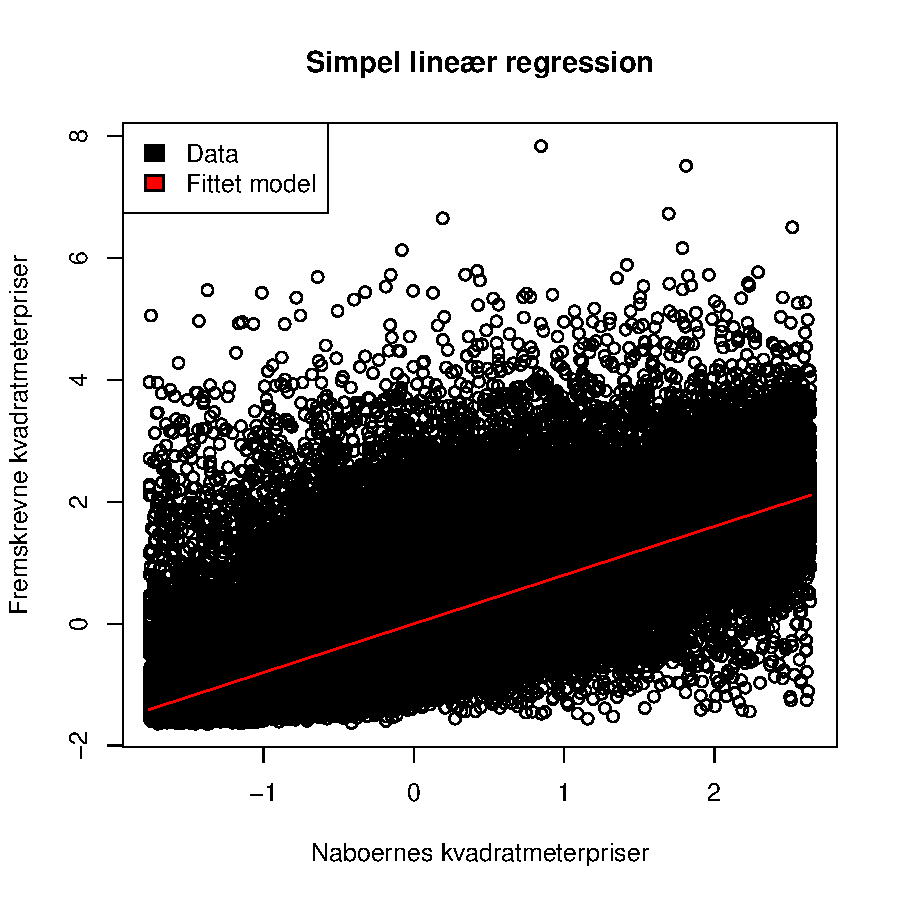
\includegraphics{rapport_latex-007}

Den anden lineære model der fittes er en multivariate lineær regressionsmodel. 
Variablene som bliver brugt i modellen er områdepriser i form af naboernes kvadratmeterpriser. Det er boligens opførelsesalder og ombygningsår, og det er boligens og grundens areal. 
I en multivariate lineær regressionsmodel kan man ikke på samme måde plotte den fittede model på det todimensionelle plot. Her kan man i stedet estimerer hvor godt modellen fitter til data ved at minimere summen af de kvadrerede afvigelser (RSS). 
Der findes flere forskellige typer af algoritmer hvis formål er at finde de parametre/vægte som laver det bedste fit til data ved at minimerer 'cost'. 

\begin{Schunk}
\begin{Soutput}
  fremskreven_pris_M2  predicted  residuals
1           0.9571538  0.5640135  0.3931403
2          -0.6903684  1.5952953 -2.2856636
4          -1.3992891 -0.9897822 -0.4095069
5          -0.4448076 -0.3181251 -0.1266825
6          -1.0156162 -0.3257869 -0.6898292
8          -0.8392054 -0.6190015 -0.2202038
\end{Soutput}
\begin{Soutput}
Call:
lm(formula = fremskreven_pris_M2 ~ EV_NN_M2 + bolig_areal + aux.ice_info.jordstykker.registreretareal_fratrukket_vejareal + 
    bolig_alder + bolig_alder, data = train)

Residuals:
    Min      1Q  Median      3Q     Max 
-5.5851 -0.2914  0.0178  0.3322  3.5360 

Coefficients:
                                                                Estimate
(Intercept)                                                    3.834e-15
EV_NN_M2                                                       8.010e-01
bolig_areal                                                   -8.561e-02
aux.ice_info.jordstykker.registreretareal_fratrukket_vejareal  8.883e-03
bolig_alder                                                   -1.371e-01
                                                              Std. Error
(Intercept)                                                    1.352e-03
EV_NN_M2                                                       1.363e-03
bolig_areal                                                    1.378e-03
aux.ice_info.jordstykker.registreretareal_fratrukket_vejareal  1.369e-03
bolig_alder                                                    1.360e-03
                                                               t value Pr(>|t|)
(Intercept)                                                      0.000        1
EV_NN_M2                                                       587.889  < 2e-16
bolig_areal                                                    -62.144  < 2e-16
aux.ice_info.jordstykker.registreretareal_fratrukket_vejareal    6.487 8.76e-11
bolig_alder                                                   -100.860  < 2e-16
                                                                 
(Intercept)                                                      
EV_NN_M2                                                      ***
bolig_areal                                                   ***
aux.ice_info.jordstykker.registreretareal_fratrukket_vejareal ***
bolig_alder                                                   ***
---
Signif. codes:  0 '***' 0.001 '**' 0.01 '*' 0.05 '.' 0.1 ' ' 1

Residual standard error: 0.5815 on 185013 degrees of freedom
Multiple R-squared:  0.6618,	Adjusted R-squared:  0.6618 
F-statistic: 9.052e+04 on 4 and 185013 DF,  p-value: < 2.2e-16
\end{Soutput}
\begin{Soutput}
[1] 0.3381834
\end{Soutput}
\end{Schunk}
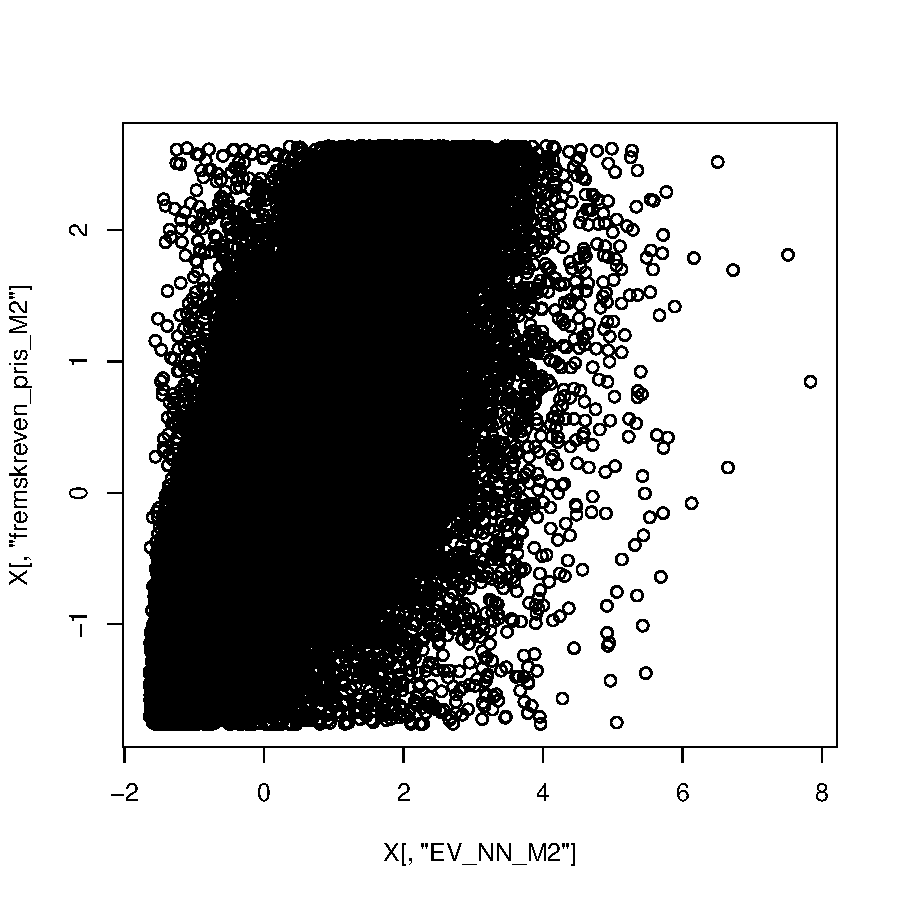
\includegraphics{rapport_latex-008}

Evalueringen af den lineære model kan foregå ved at man træner på et datasæt og prædikterer på et andet. I følgende regression har jeg nabokvadratmeterpriserne og boligarealet med som prediktorvariable. 
Ud fra den estimerede model kan man plotte sin afhængige variabel mod de predikterede værdier.
Forskellen mellem den faktiske afhænge variabel (i dette tilfælde de fremskrevne salgspiser) og den prædikterede variabel (modellens estimerede y) er residualet.
Selve den lineære regressionsmodel kan anvanceres ved at tranformere inputvariablene. Det kan eksempelvis være at opløfte variablene i anden potens og bruge dem som prediktor sammen med den originale version af variablen.
Målet for denne simple lineære regressionsmodel er reducere 'cost-funktionen' så meget som muligt. For en simpel lineær regressiosmodel er cost-funktionen en squared error, hvilket vil sige at målet her er at reducere 'mean squared error' så meget som muligt - dog uden at overfitte. 
Andre cost-funktioner kan bruges til andre problemstillinger. En logistisk funktion kan således bruges til at hvis man arbejder med et logistisk regressionsproblem. 

Ridge regression - ridge regression er regressionsmetode som bruges for at undgå at man overfitter. Overfitting sker når den fittede model fitter træningsdata rigtig godt, men at den model der trænes ikke generalisere godt på ukendt data. Overfitting kan ske både hvis der er for mange prædiktor variable eller for få observationer. 
Et godt fit er kendetegnet ved et lav RSS, men også størrelsen på koeffiecienterne - disse to til sammen udgør den samlede 'cost'. I ridge regression bruges l2-normen som et mål for størrelsen på koefficienterne og målet med ridge regression er minimere den samlede 'cost'.
Dette kan gøres ved at indføre en regulariseringsparameter (lambda), og den kan bruges til at styre kompleksisteten af sin model. 

\end{document}
